\documentclass[russian, 14pt]{beamer}
%\documentclass[handout]{beamer} %раздаточный материал
%\documentclass[aspectratio=169]{beamer}

%%% Работа с русским языком
\usepackage{cmap} %поиск в PDF
\usepackage{mathtext} %русские буквы в формулах
\usepackage[T2A]{fontenc} %кодировка
\usepackage[utf8]{inputenc} %кодировка исходного текста
\usepackage[english,russian]{babel} %локализация и переносы

%%Beamer по-русски
\newtheorem{rtheorem}{Теорема}
\newtheorem{rproof}{Доказательство}
\newtheorem{rexample}{Пример}

%%% Матпакеты
\usepackage{amsmath,amsfonts,amssymb,amsthm,mathtools} %AMS
\usepackage{icomma} %"Умная запятая": $0,2$ --  число, $0, 2$ -- перечисление

%% Номера формул
%\mathtoolsset{showonlyrefs=true} %Показывать номера только у тех в формул,
%на которые есть \eqref{} в тексте
%\usepackage{legno} %нумеризация формул слева

%%Свои команды
\DeclareMathOperator{\sgn}{\mathop{sgn}}

%%Перенос знаков в формулах (по Львовскому)
\newcommand*{\hm}[1]{#1\nobreak\discretionary{}
	{\hbox{$\mathsurround=0pt #1$}}{}}

%%%Работа с картинками
\usepackage{graphics} %Для вставки рисунков
\graphicspath{{images/}} %папки с картинками
\setlength\fboxsep{3pt} %отступ рамки \fbox{} от рисунка 
\setlength\fboxrule{1pt} %толщина линий рамки \fbox{}
\usepackage{wrapfig} %обтекание рисунков и таблиц текстом

%%%Работа с таблицами
\usepackage{array,tabularx,tabulary,booktabs} %дополнительная работа с таблицами
\usepackage{longtable} %длинные таблицы
\usepackage{multirow} %слияние строк в таблице

%%%Работа с видео и аудио
\usepackage{multimedia}
\usepackage{media9}
\usepackage{hyperref}

%%%Листинг кода
\usepackage{listings}
\usepackage{xcolor}

%%%Цвет таблиц
\usepackage{colortbl}

\definecolor{codegreen}{rgb}{0,0.6,0}
\definecolor{codegray}{rgb}{0.5,0.5,0.5}
\definecolor{codepurple}{rgb}{0.58,0,0.82}
\definecolor{backcolour}{rgb}{0.95,0.95,0.92}
\definecolor{Mycolor1}{HTML}{00F9DE}
\definecolor{Mycolor2}{HTML}{FFCCFF}
\definecolor{Mycolor3}{HTML}{990000}

\lstdefinestyle{mystyle}{
	backgroundcolor=\color{backcolour},   
	commentstyle=\color{codegreen},
	keywordstyle=\color{magenta},
	numberstyle=\normalsize\color{codegray},
	stringstyle=\color{codepurple},
	basicstyle=\ttfamily\normalsize,
	breakatwhitespace=false,         
	breaklines=true,                 
	captionpos=b,                    
	keepspaces=true,                 
	numbers=left,                    
	numbersep=5pt,                  
	showspaces=false,                
	showstringspaces=false,
	showtabs=false,                  
	tabsize=2
}

\lstset{style=mystyle}

\usepackage{caption}

\usetheme{Rochester} %тема оформления
%beamer theme matrix
\usecolortheme{whale}

\setbeamertemplate{navigation symbols}{} %отключение значков навигации

\newcommand{\cm}[1]{{\color{Mycolor3}\textbackslash#1}}

%%%Заголовок
\author[]{Панчишин Д.И.
\and Носков Р.И.
\and Пасютин А.С.
}
\title[Презентация]{Проект \textbf{«\LaTeX»}}
\subtitle{Выполнили студенты 1 курса, ФИТ-204:}
\date[]{}
\institute[]{\normalsize\textbf{КемГУ}}

\begin{document}
	
	\begin{frame}
		\maketitle
	\end{frame}

\section{Цели}

\begin{frame}
	\frametitle{\insertsection}
	\begin{itemize}
		\item Научиться делать документы с высококачественной версткой текста и формул
		\item Продемонстрировать группе возможности \LaTeX'а
	\end{itemize}
\end{frame}

\section{Задачи}

\begin{frame}
	\frametitle{\insertsection}
	\begin{itemize}
		\item Изучение инструментов и макропакетов \TeX’а
		\item Получение навыков верстки текста в \LaTeX'е
		\item Создание отчета по проекту в системе \LaTeX
	\end{itemize}
\end{frame}

\section{Индивидуальные задачи}

\begin{frame}
	\frametitle{\insertsection}
	\begin{enumerate}
		\item<1-> \textbf{Панчишин Даниил} - Тим-лид, создание тех задания, работа в \LaTeX’е с мат. формулами, рисунками и графиками;
		\item<2-> \textbf{Носков Роман} - Работа в \LaTeX’е с инструментами для верстки текста;
		\item<3-> \textbf{Пасютин Александр} - Работа в \LaTeX’е с инструментами для работы с презентациями.
	\end{enumerate}
\end{frame}

\section{Календарный план}

\begin{frame} \label{tab}
	\frametitle{\insertsection}
	\small{
	\begin{tabular}{|l|p{8,5cm}|}
		\hline
		\rowcolor{Mycolor1}
		18.02 & Распределение ролей, создание удаленного репозитория, составление календарного плана \\
		\hline
		\rowcolor{Mycolor2}
		4.03 & Изучение общего теоретического материала \\
		\hline
		\rowcolor{Mycolor1}
		18.03 & Начало работы над практической частью проекта \\
		\hline
		\rowcolor{Mycolor2}
		01.04 & Изучение отдельных аспектов \LaTeX’а, распределенных по ролям \\
		\hline
		\rowcolor{Mycolor1}
		15.04 & Создание презентации в \LaTeX, которая бы демонстрировала изученные навыки \\
		\hline
		\rowcolor{Mycolor2}
		29.04 & Создание отчета в \LaTeX, который бы демонстрировал изученные навыки
		\\
		\hline
		\rowcolor{Mycolor1}
		13.05 & Презентация результатов работы над проектом \\
		\hline
		\rowcolor{Mycolor2}
		27.05-31.05 & Защита проекта \\
		\hline
	\end{tabular}
	\hyperlink{button}{\beamerbutton{Вернуться обратно}}
}
\end{frame}

\section{Используемые средства}

\begin{frame}
	\frametitle{\insertsection}
\begin{figure}[h]
	\begin{center}
		\begin{minipage}[h]{0.4\linewidth}
			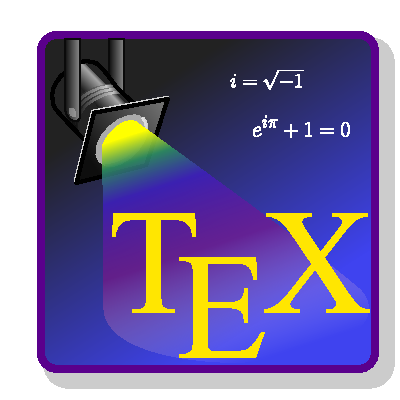
\includegraphics[width=5cm,height=5cm]{tex}
			\caption*{\huge{TeXStudio}}
		\end{minipage}
		\hfill											
		\begin{minipage}[h]{0.4\linewidth}
			
\includegraphics[width=5cm,height=5cm]{miktex}
			\caption*{\huge{MiKTeX}}
		\end{minipage}
	\end{center}
\end{figure}
\end{frame}

\section{Зачем использовать \TeX  для создания презентаций?}

\begin{frame}
	\frametitle{\insertsection}
	\begin{itemize}
		\item На слайдах отображаетя материал, набранный изначально в \LaTeX'е. 
		\item На слайдах много формул.
		\item Вам не хочется думать о переносимости файлов PowerPoint между различными версиями / компьютерами. Готовый файл pdf отображается везде. 
	\end{itemize}
\end{frame}

\subsection{Beamer}

\begin{frame}
	\frametitle{\insertsubsection}
	\begin{itemize}
		\item Beamer - класс для \LaTeX'а,специально предназначенный для создания презентаций.
		\item Позволяет настраивать внешний вид, переходы и т.п.
	\end{itemize}
	\begin{block}{}
		 \cm{documentclass}[russian, 14pt]\{beamer\}
	\end{block}
\end{frame}

\section{Титульный слайд}

\begin{frame}
	\frametitle{\insertsection}
	\begin{block}{Преамбула}
		\cm{title}[short title]\{long title\}
		
		
		\cm{subtitle}[short subtitle]\{long subtitle\}
		
		
		\cm{author}[short name]\{long name\}
		
		
		\cm{date}[short date]\{long date\}
		
		
		\cm{institute}[short name]\{long name\}
		
		
		\cm{titlepage}
	\end{block}
\end{frame}

\section{Frame'ы}

\begin{frame}
	\frametitle{\insertsection}
	\begin{block}{Один кадр}
		\cm{begin}\{frame\}
		
		
		\% код \LaTeX'а или текст 
		
		
		\cm{end}\{frame\}
	\end{block}
\end{frame}

\section{Overlay'и}

\begin{frame}
	\frametitle{\insertsection}
		\begin{block}{Примеры overlay'ев}
			\pause \cm{pause}
			
			
			\only<4-> {\cm{only}<4->} 
			
			
			\uncover<3-> {\cm{uncover}<3->}
			
			
			\alt<5> {\cm{alt}<5>}{Сейчас не 5 кадр}
			
			
			\temporal<6>{Сейчас не 6 кадр}{\cm{temporal}<6>}{6 кадр уже прошел}
			
			
			\begin{itemize}
				\item<7> {\cm{item}<7>} 
			\end{itemize}
		\end{block}
\end{frame}

\section{Блоки}

\begin{frame}
	\frametitle{\insertsection}
	\begin{block}{Название блока}
		Содержимое блока
	\end{block}


	\cm{begin}\{block\}\{Название блока\}
	
	
	Содержимое блока
	
	
	\cm{end}\{block\}
\end{frame}

\section{Таблицы}

\begin{frame}
	\frametitle{\insertsection}
	\begin{flushleft}
	\cm{begin}\{tabular\}\{|l|p{8,5cm}|\}
	
	
		\cm{hline}
		
		
		18.02 \& Распределение ролей, создание удаленного репозитория, составление календарного плана \textbackslash\textbackslash
		
		
		\cm{hline}


		...
		
		
		\cm{end}\{tabular\}
		
		
		\hyperlink{tab}{\beamerbutton{Посмотреть таблицу}}
	\end{flushleft}
\end{frame}

\section{Ссылки, кнопки, рисунки}

\begin{frame} \label{button}
	\frametitle{\insertsection}
	\cm{hyperlink}\{label\}\{\cm{beamerbutton}\{Кнопка\}\}
	
	
	\cm{hyperlink}\{label\}\{\cm{includegraphics}[scale=0.3]\{kemsu\}\}
	
	
	\centering\hyperlink{video}{
\includegraphics[scale=0.3]{kemsu}}
\end{frame}

\section{Видео}

\begin{frame} \label{video}
	\frametitle{\insertsection}
	\includemedia[
	activate=pageopen,
	width=320pt,height=180pt,
	addresource=kem.mp4,
	flashvars={%
		source=kem.mp4
		&loop=true}
	]{}{VPlayer.swf}
\end{frame}

\section{Листинг кода}

\begin{frame}
	\frametitle{\insertsection}
	\begin{block}{}
		\cm{lstinputlisting}[language=C++]\{programm.cpp\}
	\end{block}
	\lstinputlisting[language=C++]{programm.cpp}
\end{frame}

\usebackgroundtemplate{
\includegraphics[width=\paperwidth,height=\paperheight]{background.jpg}}

\section{Фон}

\begin{frame}
	\frametitle{\insertsection}
	\begin{block}{}
		\cm{usebackgroundtemplate}\{
		\cm{includegraphics}\{background.jpg\}\}
	\end{block}
\end{frame}

\usebackgroundtemplate{}

\section{Свои команды}

\begin{frame}
	\frametitle{\insertsection}
	\begin{block}{}
		\cm{newcommand}\{\textbackslash имя\}[число]\{действия\}
	\end{block}
	\begin{block}{}
		\cm{newcommand}\{\textbackslash cm\}[1]\{\cm{color}\{Mycolor3\}
		\cm{textbackslash}\#1\}
	\end{block}
\end{frame}

\section{Оглавление}

\begin{frame}
	\frametitle{\insertsection}
		\tableofcontents
\end{frame}

\begin{frame}
	\frametitle{Итоговый результат}
\end{frame}
\end{document}